\documentclass[tikz,border=10pt]{standalone}

\usepackage{xcolor}
\usetikzlibrary{arrows.meta, positioning}

\definecolor{paperGreen}{RGB}{34,125,92}
\definecolor{paperSoft}{RGB}{246,248,250}
\definecolor{paperLine}{RGB}{80,92,110}

\begin{document}
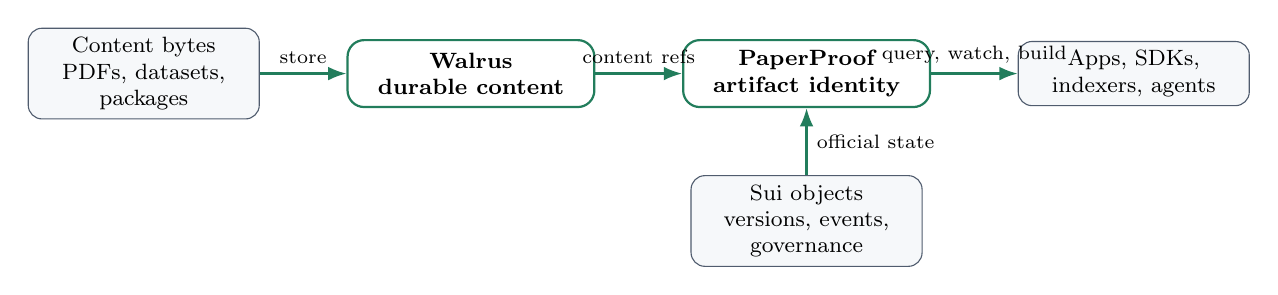
\begin{tikzpicture}[
    node distance=1.1cm,
    box/.style={draw=paperLine, rounded corners=5pt, fill=paperSoft, minimum height=0.75cm, align=center, font=\footnotesize, text width=2.7cm},
    core/.style={draw=paperGreen, thick, rounded corners=6pt, fill=white, minimum height=0.85cm, align=center, font=\footnotesize\bfseries, text width=2.9cm},
    arrow/.style={-Latex, thick, draw=paperGreen}
]
    \node[box] (content) {Content bytes\\PDFs, datasets, packages};
    \node[core, right=of content] (walrus) {Walrus\\durable content};
    \node[core, right=of walrus] (series) {PaperProof\\artifact identity};
    \node[box, right=of series] (apps) {Apps, SDKs,\\indexers, agents};
    \node[box, below=0.85cm of series] (sui) {Sui objects\\versions, events, governance};

    \draw[arrow] (content) -- node[above, font=\scriptsize] {store} (walrus);
    \draw[arrow] (walrus) -- node[above, font=\scriptsize] {content refs} (series);
    \draw[arrow] (sui) -- node[right, font=\scriptsize] {official state} (series);
    \draw[arrow] (series) -- node[above, font=\scriptsize] {query, watch, build} (apps);
\end{tikzpicture}
\end{document}
